%!TEX root = ../main.tex

\chapter{The background model before cuts}\label{chap:bkg:raw:ph2}

As already mentioned, a precise knowledge of background intensity and distribution is
essential to searches of faint signals. One main assumption of the \onbb-decay signal
analysis is the distribution of background events in the analysis window around \qbb\
being uniform, except for the known \Tl\ and \Bil\ \g\ lines. The primary role of the
background model is to verify this assumption by exploiting data outside this energy
region or filtered with a different event selection. The background model is also
complementary to assay measurements in determining the location of the most dangerous
background sources and learn how to improve experimental design and material selection in
similar future projects. Lastly, a good background model allows to isolate \nnbb-decay
events, estimate the half-life of the process and study their distribution as a source of
potential new-physics effects (see \cref{chap:theory}).
\newpar
A first background model has been built for the \phaseone\ data and published
in~\cite{Agostini2013a}. Later, a new and advanced model has been constructed to describe
the first 60~\kgyr\ of \phasetwo\ data before the LAr veto and PSD cuts, which has been
published in~\cite{Agostini2019b} and is described in detail in this chapter.

\section{Analysis data sets}%
\label{sec:bkg:raw:data}

\begin{table}[b]
  \small
  \centering
  \caption{%
    Properties of the data sets considered in this analysis. Further
    details about the \gerda\ detectors can be found in past
    publications~\cite{Agostini2013a, Agostini2018a}.
  }\label{tab:bkg:raw:ph2:datasets}
  \begin{tabular}{lccccc}
  \toprule
  \mr{2}{data set} & \mr{2}{composition}     & total Ge           & active \gesix\   & total Ge           & active \gesix\     \\
                   &                         & mass (kg)          & mass (kg)        & exposure (\kgyr)   & exposure (\kgyr)   \\
  \midrule
  \enrBEGeIIp\     & 29 \bege\footnotemark{} & $19.362 \pm 0.005$ & $17.17 \pm 0.32$ & $22.181 \pm 0.006$ & $17.31  \pm 0.32$  \\
  \enrSCoaxIIp\    & 6 \scoax\               & $11.827 \pm 0.002$ & $10.38 \pm 0.42$ & $13.179 \pm 0.003$ & $10.00  \pm 0.42$  \\
  \enrICoaxIIp\    & 4 \icoax\               & $ 7.802 \pm 0.002$ & $ 7.23 \pm 0.03$ & $ 8.775 \pm 0.002$ & $ 7.13  \pm 0.03$  \\
  \enrGeIIp\       & all enriched            & $38.991 \pm 0.006$ & $34.78 \pm 0.53$ & $44.135 \pm 0.007$ & $34.44  \pm 0.53$  \\
  \bottomrule
\end{tabular}

% vim: nowrap

\end{table}%
\footnotetext[1]{%
  The BEGe detector \GD{02D} is the only detector that does not fully
  deplete~\cite{Agostini2018a}. Hence, events triggered by this detector are
  not considered in either data set and it is omitted from the mass
  computation.
}

As already mentioned, the background model before cuts has been developed using data from
the first part of \phasetwo, namely, for data acquired starting from December 2015 to
March 2018. Single-detector (or multiplicity-one, abbreviated \Mone) events and
two-detector (multiplicity-two, abbreviated \Mtwo) events are considered for this
analysis. Events from the coaxial detectors with natural isotope composition, located in
the central detector string, are not used in this analysis due to large uncertainties on
their \nplus\ contact thickness and detection efficiency. The \Mone\ events are split in
two data sets based on the two enriched detector geometries which we call \enrBEGeII\ and
\enrCoaxII\ in the following.  The \Mtwo\ data form a third data set which is named
\enrGeII. The energy we associate to an \Mtwo\ event is the sum of the energies
reconstructed in the two detectors. The data sets, their exposure and respective detector
mass are listed in \cref{tab:bkg:raw:ph2:datasets}. Note that the \bege\ exposure of
31.1~\kgyr\ is higher than the one reported in~\cite{Agostini2019a} because additional
data for which PSD methods are not applicable is here included.

\begin{figure}
  \centering
  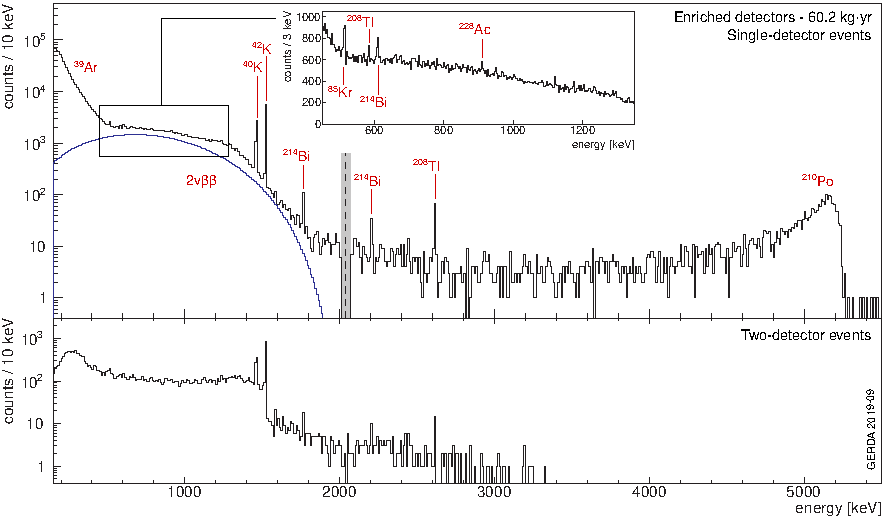
\includegraphics[width=0.9\linewidth]{plots/bkg/raw/ph2/dataGe-desc.pdf}
  \caption{%
    Summed energy spectra of single-detector events (\enrBEGeII\ and \enrCoaxII, top
    panel) and two-detector events (\enrGeII, bottom panel) collected in \gerda\
    \phasetwo.  The prominent features due to detector intrinsic \nnbb\ events, \kvz,
    \Arl\ and \Kr\ in the LAr, \kvn, the \Thh\ and \Uh\ decay chains are highlighted. The
    window blinded for the \onbb\ analysis is marked in grey.
  }\label{fig:bkg:raw:ph2:datasets}
\end{figure}

The event energy distribution of the three data sets is displayed in
\cref{fig:bkg:raw:ph2:datasets}; the sum spectrum of \enrBEGeII\ and \enrCoaxII\ in the
top panel and \enrGeII\ in the bottom panel. For the single-detector data, in the top
panel, the following features are most noticeable: the \b\ decay of \Arl\ dominates the
spectrum up to 565~keV while between 600 and 1500~keV the most prominent component is the
continuous spectrum of \nnbb\ decay of \gesix. Two \g\ lines at 1461 and 1525~keV can be
attributed to \kvn\ and \kvz; further visible \g\ lines belonging to \Kr, \Tl, \Bih\ and
\Ac\ are indicated in the figure. The highest energies displayed are dominated by a
peak-like structure emerging at 5.3~MeV with a pronounced low energy tail. This is a
typical spectral feature of \a\ particles and can, here, be attributed to \Po\ decay on
the thin detector \pplus\ surfaces~\cite{Agostini2013a}.  Events above the \Po\ peak
belong to \a\ decays emerging from the \Ra\ sub-chain on the detector \pplus\ surfaces.
All these components contribute also to \enrGeII\ except for \Arl, \nnbb\ and high energy
\a-components. This is due to the short range of \a\ (tens of \mum) and \b\
particles (typically smaller than 1.5~cm) in LAr and germanium with respect to the
distance between detectors which is of the order of several cm.

\section{Monte Carlo simulations and probability density functions}

The probability density functions (pdfs) used to model contributions to the energy spectra
are obtained from Monte Carlo simulations. The latter are performed using the \mage\
simulation framework~\cite{Boswell2011}, based on
\geant~\texttt{v10.4}~\cite{Agostinelli2002, Allison2006, Allison2016}.  \mage\ contains a
software implementation of the \gerdatwo\ detectors as well as the assembly and all other
surrounding hardware components. A visualization of this implementation is presented in
\cref{fig:setup:magevolumes}. Detector intrinsic \nnbb\ decays of \gesix\ and background
events originating from radioactive contaminations in and around the detector assembly are
simulated. The energy spectrum of the two electrons emitted in the \nnbb\ decay was
sampled according to the distribution given in~\cite{Tretyak1995} and implemented in
\decayzero~\cite{Ponkratenko2000}. The pdfs are obtained from the Monte Carlo simulations,
taking into account the finite energy resolution and individual exposure acquired with
each detector during the considered data taking periods. Special care is taken not to
statistically bias the pdfs by assuring that each simulated decay is taken into account
only once in the production of a pdf. For more details see \cref{apdx:magepdfs}.

\section{Background expectation}%
\label{sec:bkg:raw:ph2:priors}

The structural components of the setup have been screened for their radio-purity before
deployment. Two measurement methods were used depending on the screened isotope: \g-ray
spectroscopy (Ge-\g) with High Purity Germanium (in four underground laboratories, for
details see reference~\cite{Ackermann2012}) and mass spectrometry with Inductively Coupled
Plasma Mass Spectrometers (ICP-MS)~\cite{Vacri2015}. Especially materials close to the
detectors have been screened for radioactive contaminations originating from the \Uh\ and
\Thh\ decay chains, \kvn\ and \Co. For measured activities and upper limits see
reference~\cite{Agostini2018a} Sec.~5. All possible background sources taken into
consideration in this analysis are described in detail below. The descriptions are
accompanied by a selection of pdfs in \cref{fig:bkg:raw:ph2:pdfs:gmodel} (see also
\cref{apdx:magepdfs}).

\blocktitle{\Thh\ \\ \Uh}
The only isotopes simulated are \Pa, \Pbh\ and \Bih\ from the \Uh\ decay chain and \Ac,
\Bil\ and \Tl\ from the \Thh\ decay chain. The following groups of isotopes are assumed to
be in secular equilibrium: [\Uh, \Pa] [\Ra, \Pbh, \Bih] [$^{228}$Ra, \Ac] and [\Th, \Bil,
\Tl]. Their decay products consist of \g\  or \b\ particles with an energy higher than
520~keV. Less energetic particles from the remaining constituents in the chain do not
enter the energy window which is considered in the presented analysis. The \a\ emitters
from the decay chains contaminating the thin \pplus\ electrodes are described below.

\blocktitle{\Co}
A significant fraction of components in the \gerda\ setup is made of
copper~\cite{Agostini2018a}, which can be produced with high radio-purity but is
potentially activated by cosmic rays producing the long-lived isotope \Co. The latter
decays with a half-life of 5.2711(8)~yr; from material screening it is also expected to be
found in some of the detector high-voltage flexible flat cables.

\blocktitle{\kvn}
This isotope is found in all screened materials.  Construction materials were not
optimized for ultra-low \kvn\ content because the Q-value of its decay is well below \qbb\
and hence does not contribute to the background in the ROI. The \kvn\ decay spectrum
exhibits a \g\ line at 1460.822(6)~keV with an accumulated statistics on the order of
100~cts/detector. In \cref{fig:bkg:raw:ph2:pdfs:kmodel} the expected counts per detector
channel for \kvn\ simulated in different locations are shown. Using the ratio of events
detected in different detectors, information about the spatial distribution of \kvn\ can
be extracted. We use this spatial information to resolve degeneracies of \kvn\ in the
energy spectra (for details see \cref{apdx:kmodel}).

\blocktitle{\kvz}
A cosmogenically produced isotope in LAr is \Arh\ ($T_{1/2} = 32.9(11)$~yr) which decays
to \kvz. The distribution of \kvz\ inside the LAr is likely to be inhomogeneous due to
drift of the ionized decay products induced by the electric field (generated by
high-voltage cables and detectors) and convection. \kvz\ decays to $^{42}$Ca via \b\ decay
with a half-life of 12.355(7)~h and a Q-value of 3525.22(18)~keV, well above \qbb. For the
\b\ particle to be detected the decay needs to happen within a distance of a few
centimeters\footnote{The path length of \kvz\ \b\ particles in LAr is less than 1.6~cm,
but bremsstrahlung photons from the interaction with LAr can travel as far as
$\sim$10~cm.} to the detector surface. As the detectors are in direct contact with the
LAr, the \b\ component of \kvz\ potentially gives one of the most significant
contributions to the background in the ROI. Therefore, we separate decays originating
inside and outside the mini-shrouds in the following analysis. The full-range fit has
little sensitivity to any potassium inhomogeneity outside the mini-shrouds. \kvz\ is hence
assumed to be distributed homogeneously in this region. Based on detector-wise
observations, however, a surplus of \kvz\ above the detector array in the vicinity of the
front-end electronics is deduced (see \cref{apdx:kmodel}). Inside the mini-shrouds the \b\
spectrum becomes potentially important.  Some scenarios are possible, the closer \kvz\
decays to the detector surface, namely to the \nplus\ and \pplus\ contacts, the more \b\
particles enter the germanium. A fraction of events around \qbb\ coming from \kvz\ is
potentially due to \g\ particles with higher energy and sub-percent level branching ratio
or simultaneous energy deposition of multiple \g\ particles. This \g\ component could
become important for large quantities of \kvz\ not located directly on the detector
surfaces with the \b\ particle being absorbed in the LAr. As for \kvn\ also the \g\ line
at 1525~keV of \kvz\ contains valuable information about the spatial decay distribution of
this isotope. In contrast to \kvn\ no additional information, e.g.~from radio-purity
screening measurements, is available. For more detailed information about \kvn\ and \kvz\
see \cref{apdx:kmodel}.

\blocktitle{\a\ emitters}
The lithium-diffused \nplus\ detector surfaces act as a barrier for \a\ particles. The
latter can only penetrate the very thin boron-implanted \pplus-contact or the contact
separating groove. \a\ particles have to be emitted directly at the surface or from a thin
adjacent layer of LAr. Since \a\ particles have to cross the $\sim 0.5$~\mum\ thick
\pplus\ dead layer and therefore only part of their initial energy is deposited in the
active volume, this background component leads to peaks with characteristic low-energy
tails in the HPGe energy spectra (see \cref{fig:bkg:raw:ph2:pdfs:amodel:Po}). Some \a\
events, presumably originating from the detector groove, are reconstructed with degraded
energy and lead to an additional, continuous spectral component. We find mainly \Po\ but
also traces of isotopes from the \Ra\ decay chain.

\blocktitle{Detector bulk \\ impurities}
Cosmogenically produced long-lived isotopes can also be found in
germanium~\cite{Meierhofer2009, Meierhofer2010, Meierhofer2012}. In particular, $^{68}$Ge
and \Co\ can occur as detector intrinsic impurities with half-lives of 270.93(13)~d and
5.2711(8)~yr.  The \bege\ detectors were kept underground during major parts of the
fabrication and characterization operations. Periods when these detectors were above
ground have been tracked in a database~\cite{Agostini2015e}.  Thus, for the well-monitored
BEGe detectors we expect impurities of 5~nuclei/kg of $^{68}$Ge and 21~nuclei/kg of \Co\
as of September 2014~\cite{Agostini2015e}. Extrapolating the expected impurities to the
whole \phasetwo\ data taking period we expect on average 0.03~cts/day from $^{68}$Ge and
0.1~cts/day due to \Co. From background modeling in Phase I~\cite{Agostini2013a} the
contribution for the coaxial detectors formerly used in the Heidelberg-Moscow
(\hdm)~\cite{Klapdor2001} and \igex~\cite{Aalseth2002} experiments is expected to be even
smaller due to their long storage underground. Simulating the expected detector bulk
impurities we find background contributions around \qbb\ of less than $10^{-4}$~\ctsper\
in both cases. Hence, we conclude that $^{68}$Ge as well as \Co\ can be neglected in the
following analysis. Potential bulk contaminations with \Uh\ and \Thh\ were studied in
reference~\cite{Agostini2016a}. Only upper limits were found, establishing germanium
crystals as material of outstanding radio-purity.  Hence, we only consider the decay of
\gesix\ via \nnbb\ as detector intrinsic background component while all other intrinsic
impurities are considered to be negligible.

\blocktitle{Other sources}
As discussed in reference~\cite{Agostini2013a}, prompt cosmic muon induced background
events are efficiently vetoed by the identification of \v{C}erenkov light emitted by muons
when they pass the water tank. The expected BIs, due to the direct muon and neutron fluxes
at the LNGS underground laboratory, have been estimated to be of the order
$3\cdot10^{-5}$~\ctsper~\cite{Freund2014} and $10^{-5}$~\ctsper~\cite{Meierhofer2012} in
earlier works, respectively.  Background contributions coming from delayed decays of
$^{77}$Ge and $^{77\text{m}}$Ge, also induced by cosmic muons, are estimated to be
$0.21\pm0.01$~nuclei/(kg$\cdot$yr)~\cite{Wiesinger2018} corresponding to a BI prior to the
active background suppression techniques of about $10^{-5}$~\ctsper. Also, the water tank
and LAr cryostat contaminations are expected to contribute to the \gerda\ BI with less
than $10^{-4}$~\ctsper~\cite{Ackermann2012, Barabanov2009}. All above mentioned
contributions are considered negligible in this work. Other potential sources of
background from interactions of \gesix~\cite{Meierhofer2012, Vanhoefen2018} and
$^{206}$Pb~\cite{Mei2007} with neutrons and $^{56}$Co for which no evidence was found are
not taken into consideration. The cosmogenically produced isotope \Arl\ and the
anthropogenic isotope \Kr~\cite{Winger2005}, which are dissolved in LAr, emit particles
which are dominantly less energetic than the energy window which is considered in the
presented analysis.

\begin{figure}[p]
  \centering
  \subfloat[%
    \Co, \Pa, \Ac\ contaminations and detector intrinsic \nnbb\
    decay.\label{fig:bkg:raw:ph2:pdfs:gmodel:other}%
  ]{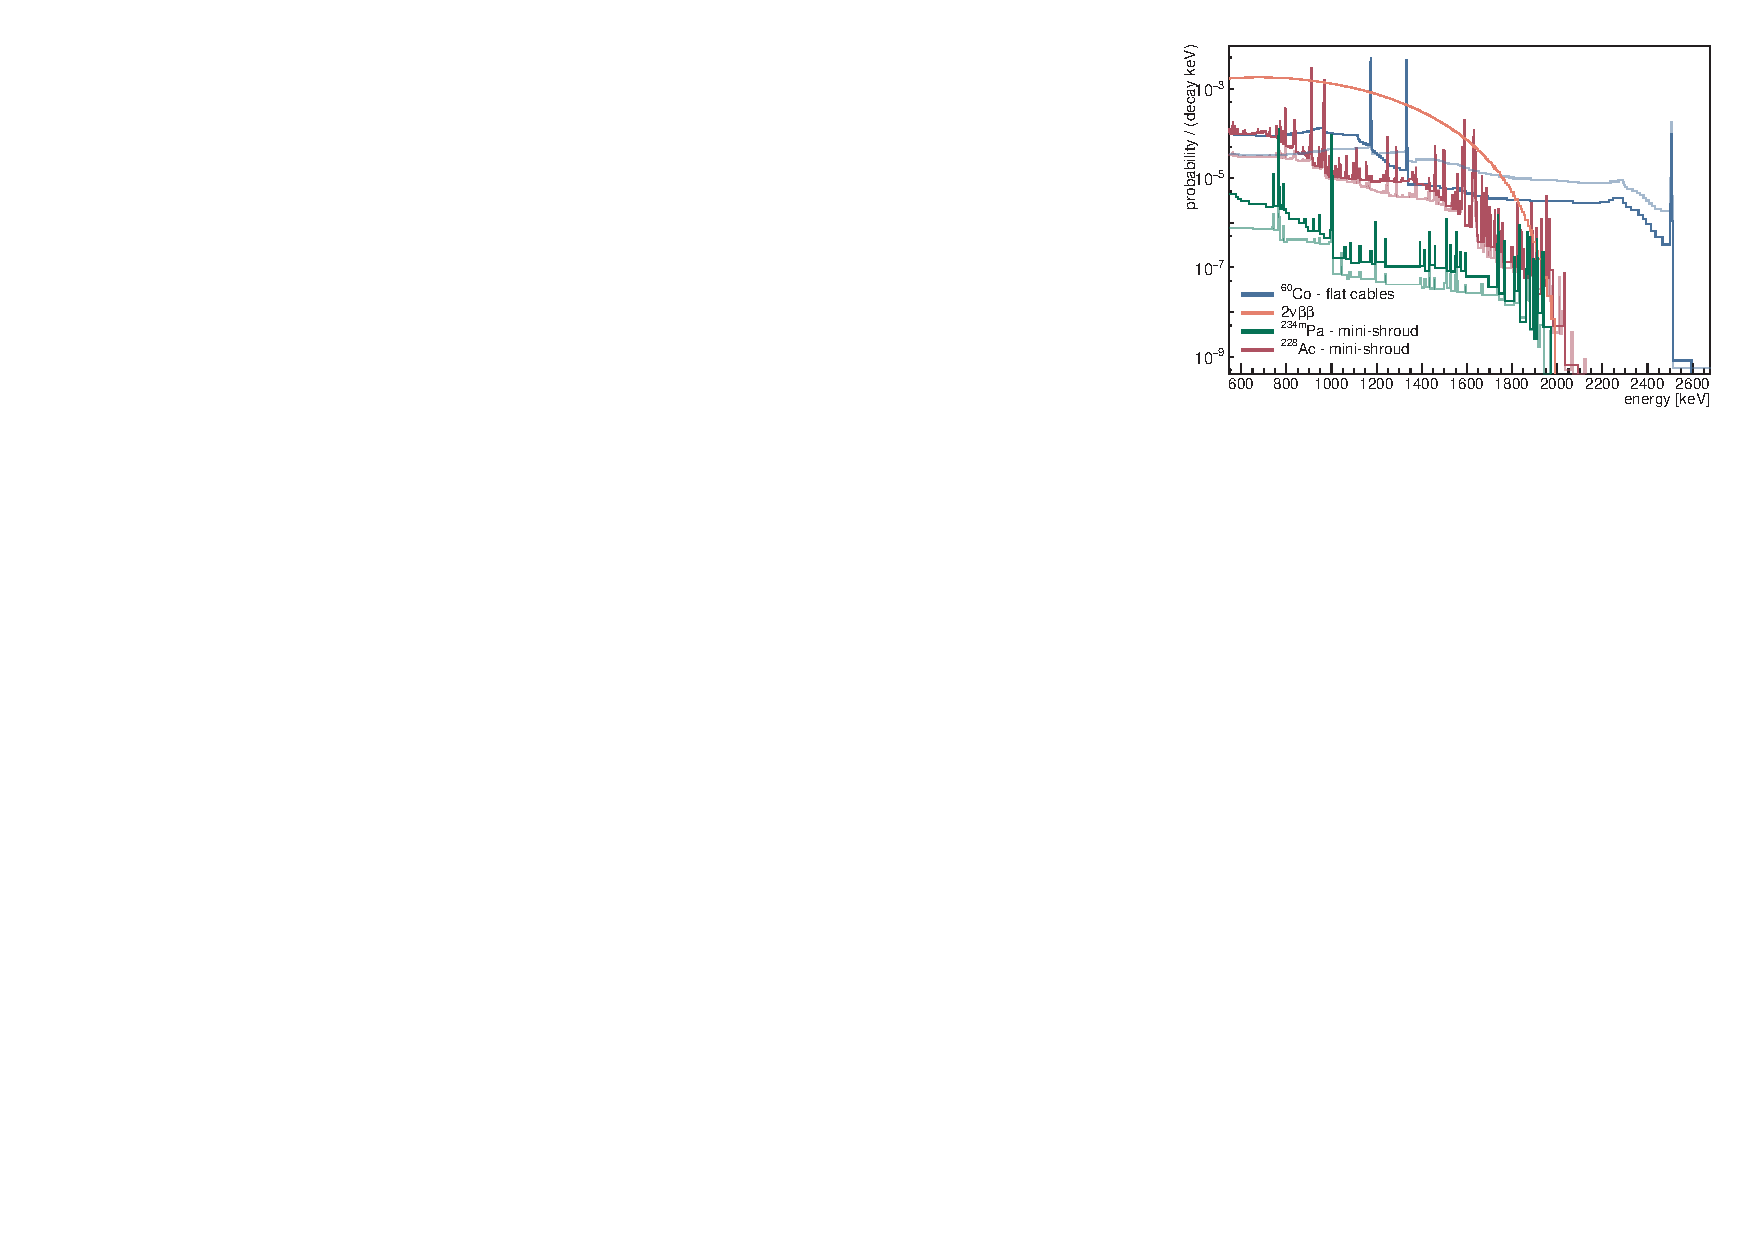
\includegraphics[width=0.45\textwidth]{plots/bkg/raw/ph2/pdfs/gmodel-pdfs-misc.pdf}}
  \hspace{10pt}
  \subfloat[%
    \Bil\ and \Tl\ (\Thh\ chain) contaminations far from (fiber shroud)
    and close to (mini-shrouds) the detector
    array.\label{fig:bkg:raw:ph2:pdfs:gmodel:Th}%
  ]{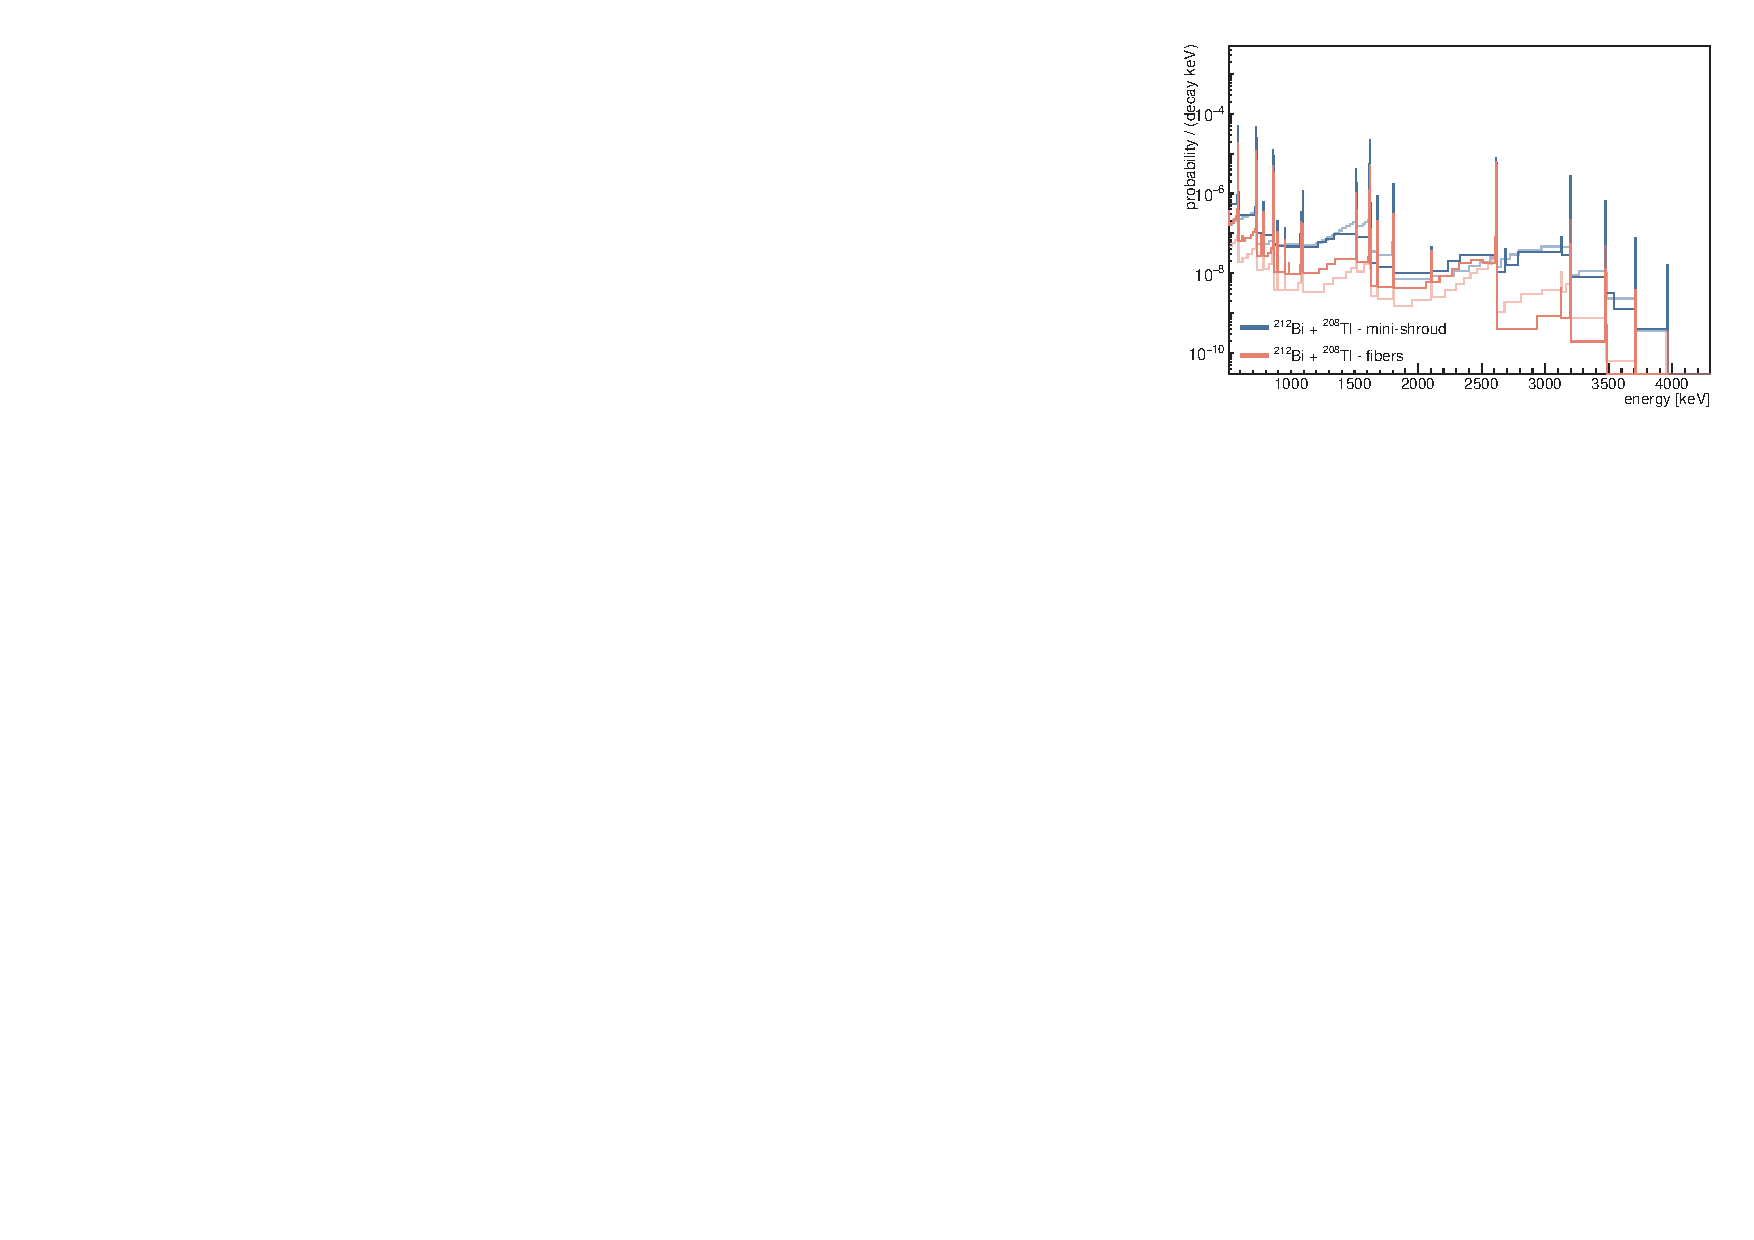
\includegraphics[width=0.45\textwidth]{plots/bkg/raw/ph2/pdfs/gmodel-pdfs-Th.pdf}} \\
  \subfloat[%
    \kvn\ contamination close to the detector array (on the
    mini-shrouds), at a higher radial distance (on the fiber shroud) and
    higher vertical distance (on the copper
    shrouds).\label{fig:bkg:raw:ph2:pdfs:gmodel:K40}%
  ]{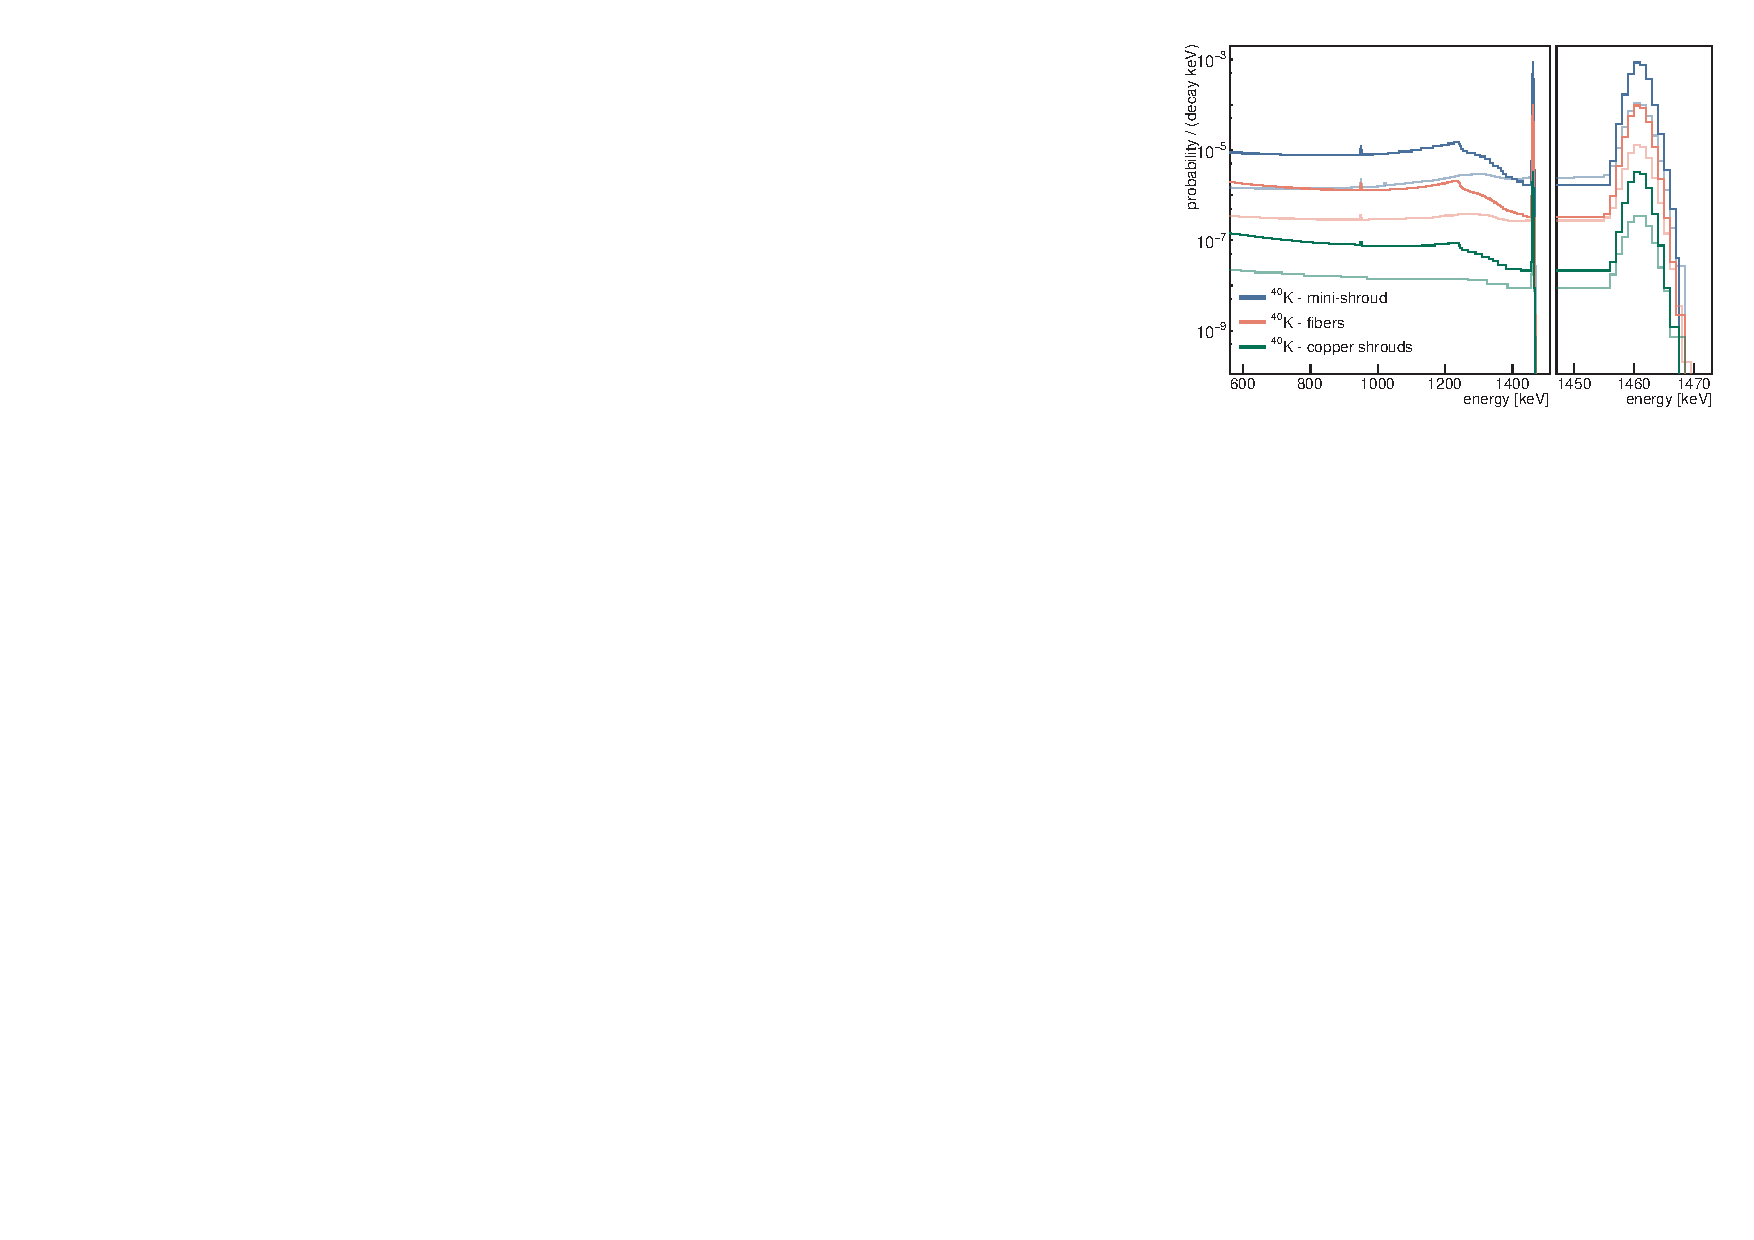
\includegraphics[width=0.45\textwidth]{plots/bkg/raw/ph2/pdfs/gmodel-pdfs-K40.pdf}}
  \hspace{10pt}
  \subfloat[%
    \kvz\ contamination in different locations inside the
    LAr.\label{fig:bkg:raw:ph2:pdfs:gmodel:K42}%
  ]{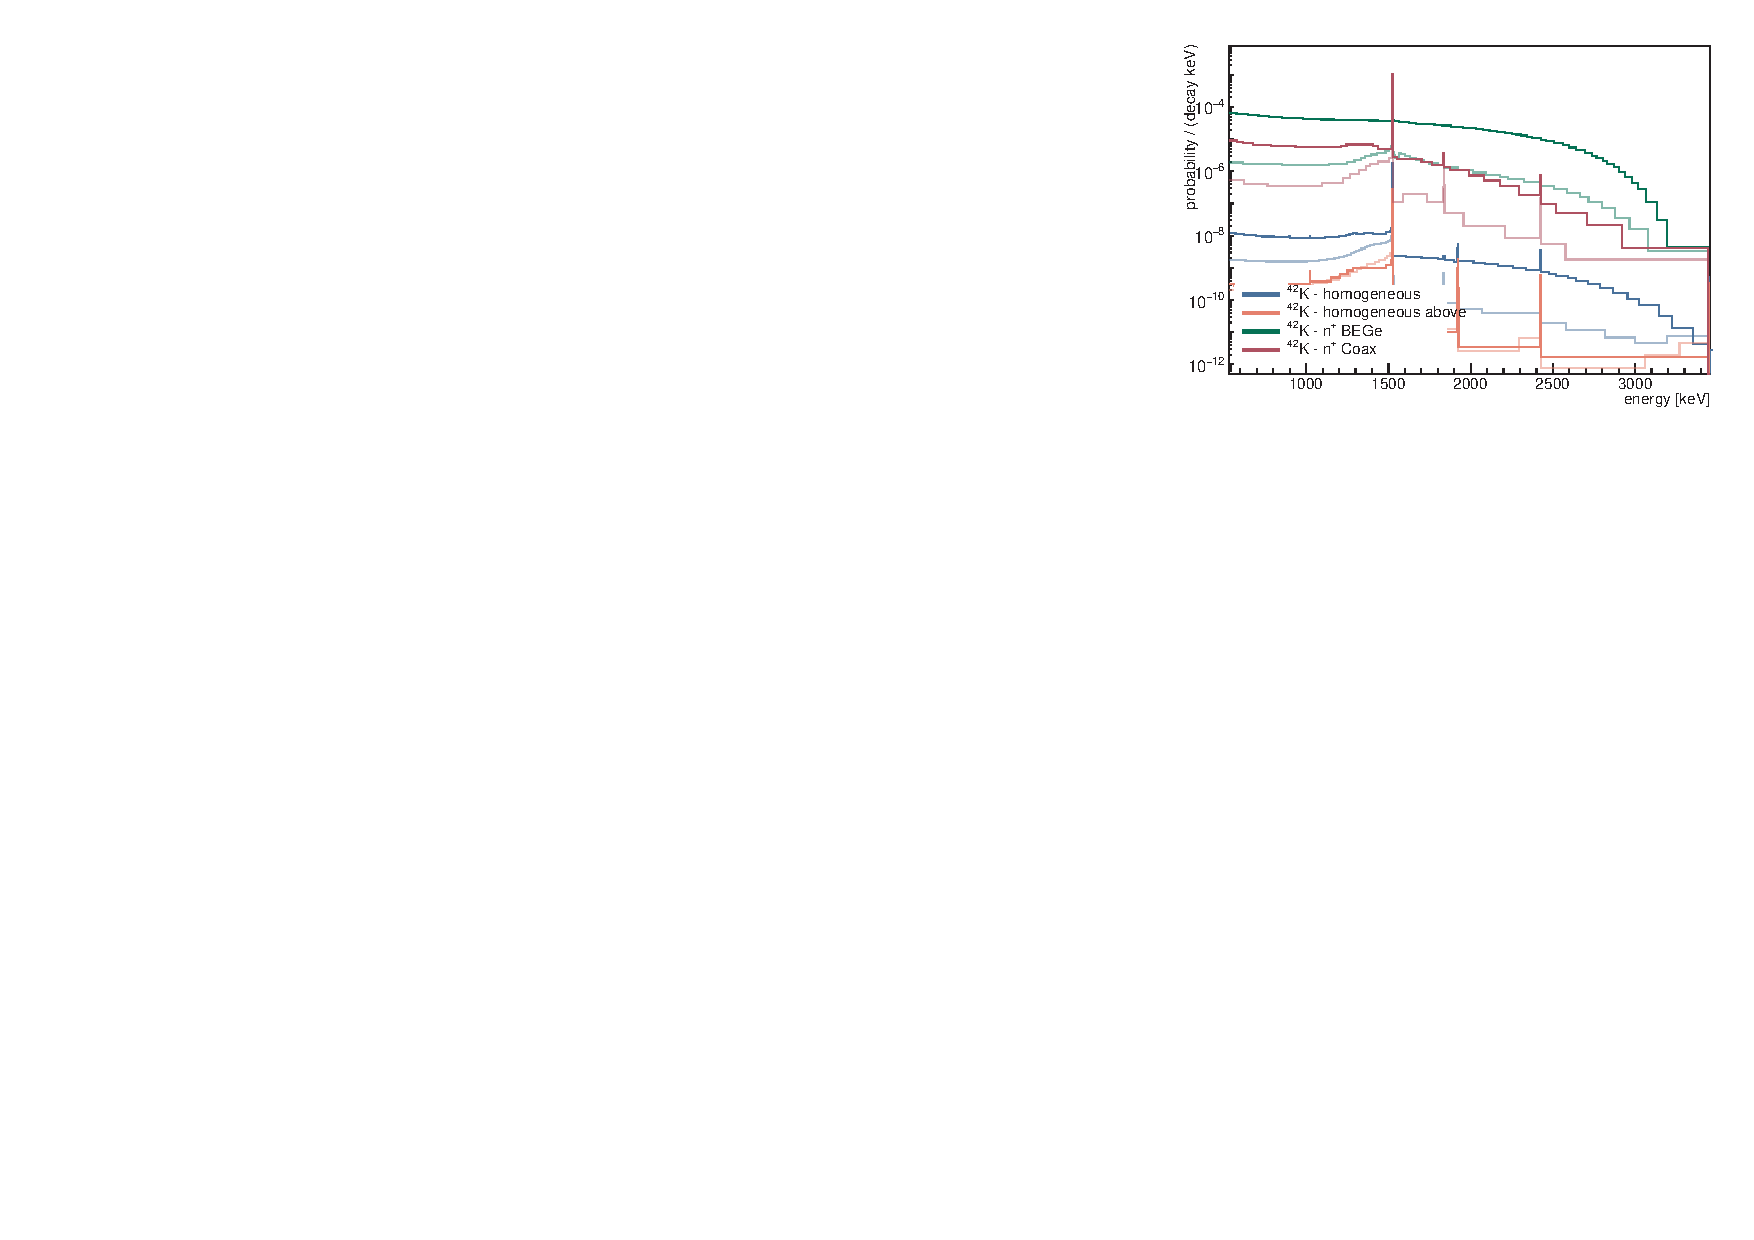
\includegraphics[width=0.45\textwidth]{plots/bkg/raw/ph2/pdfs/gmodel-pdfs-K42.pdf}} \\
  \subfloat[%
    \Po\ \a\ decays on \pplus\ contact surface for different
    thicknesses of the inactive contact layer. For 0~nm the nuclear
    recoil energy can be absorbed and some energy can be lost in the
    LAr.\label{fig:bkg:raw:ph2:pdfs:amodel:Po}%
  ]{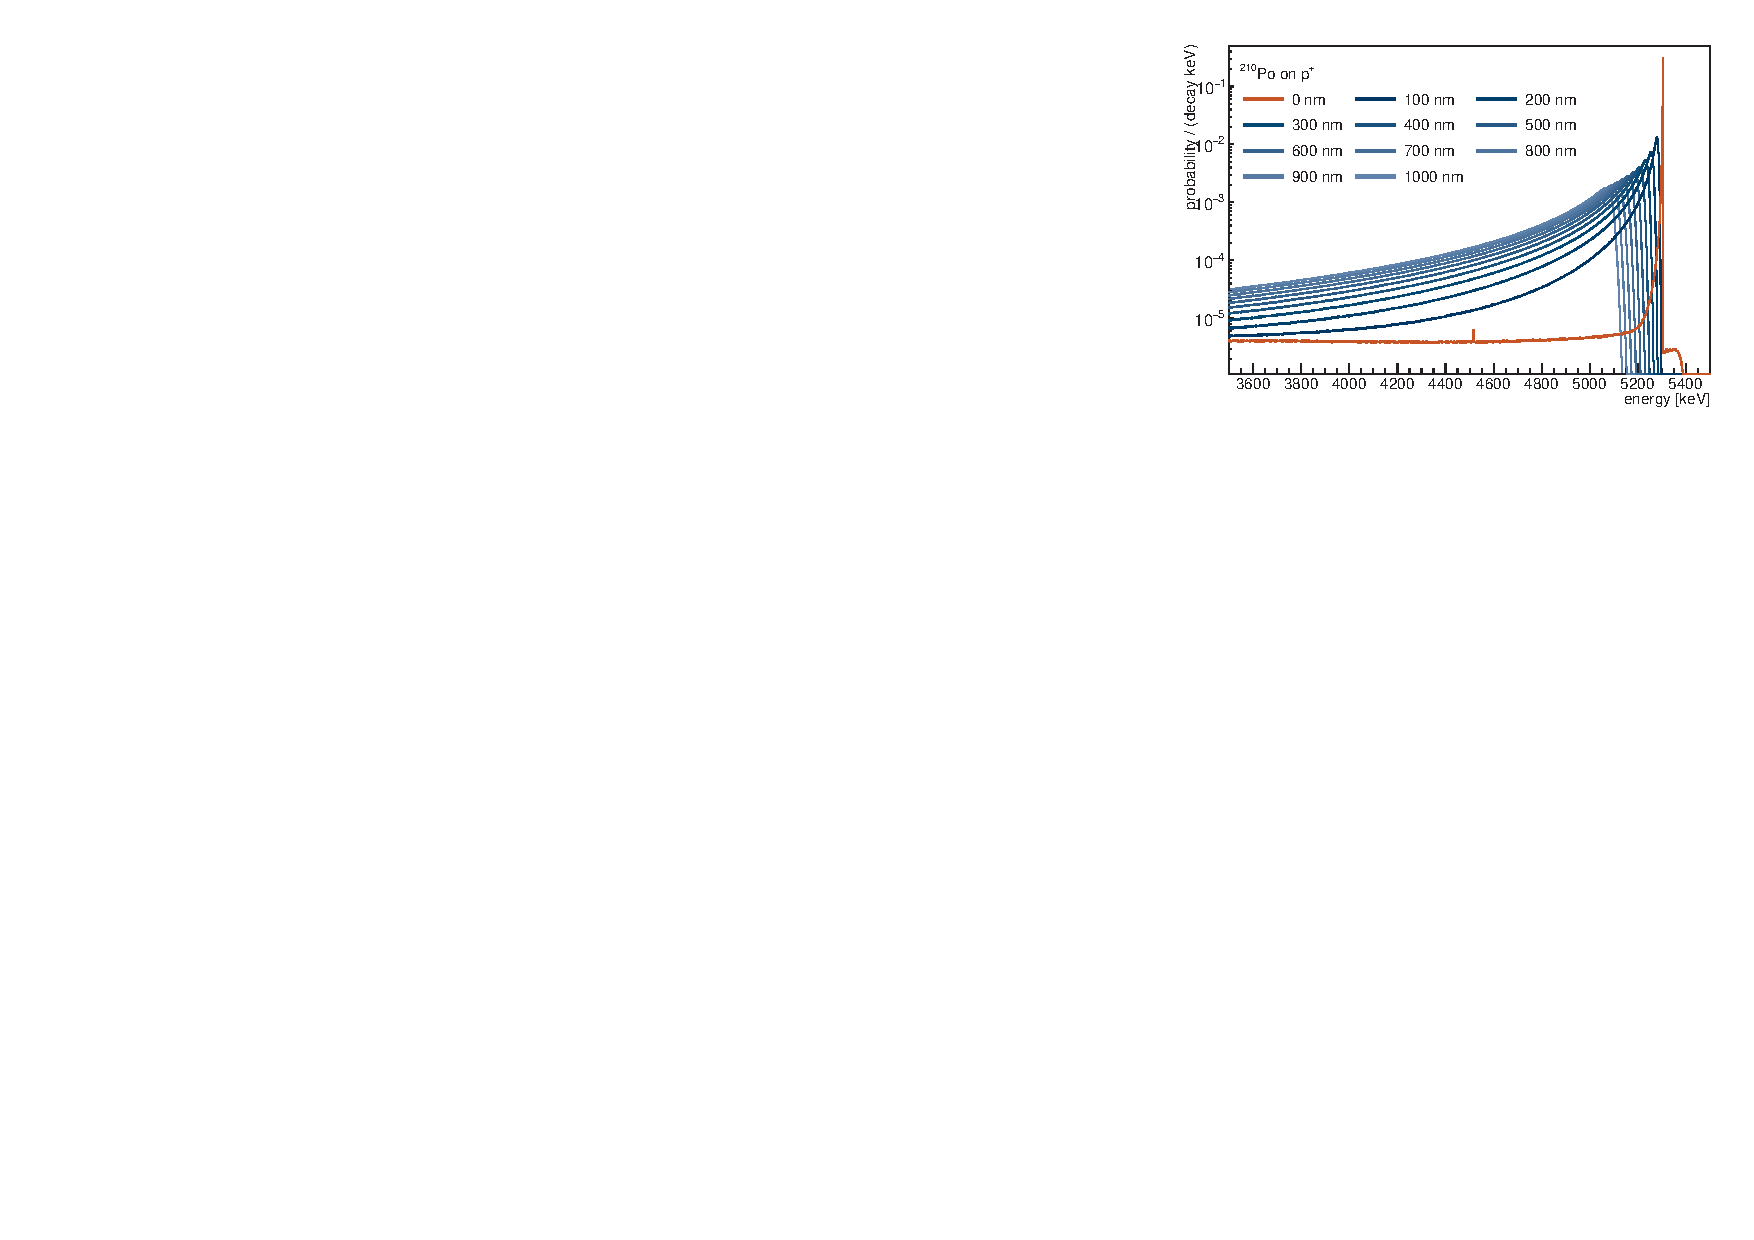
\includegraphics[width=0.45\textwidth]{plots/bkg/raw/ph2/pdfs/amodel-pdfs-Po210.pdf}}
  \hspace{10pt}
  \subfloat[%
    \kvz\ contamination in different volumes in the LAr and detector
    intrinsic \nnbb\ for comparison. The energy window (ROI) considered
    is \mbox{$(1525\pm4)$~keV} (\kvz\ \g\ line).\label{fig:bkg:raw:ph2:pdfs:kmodel:K42}%
  ]{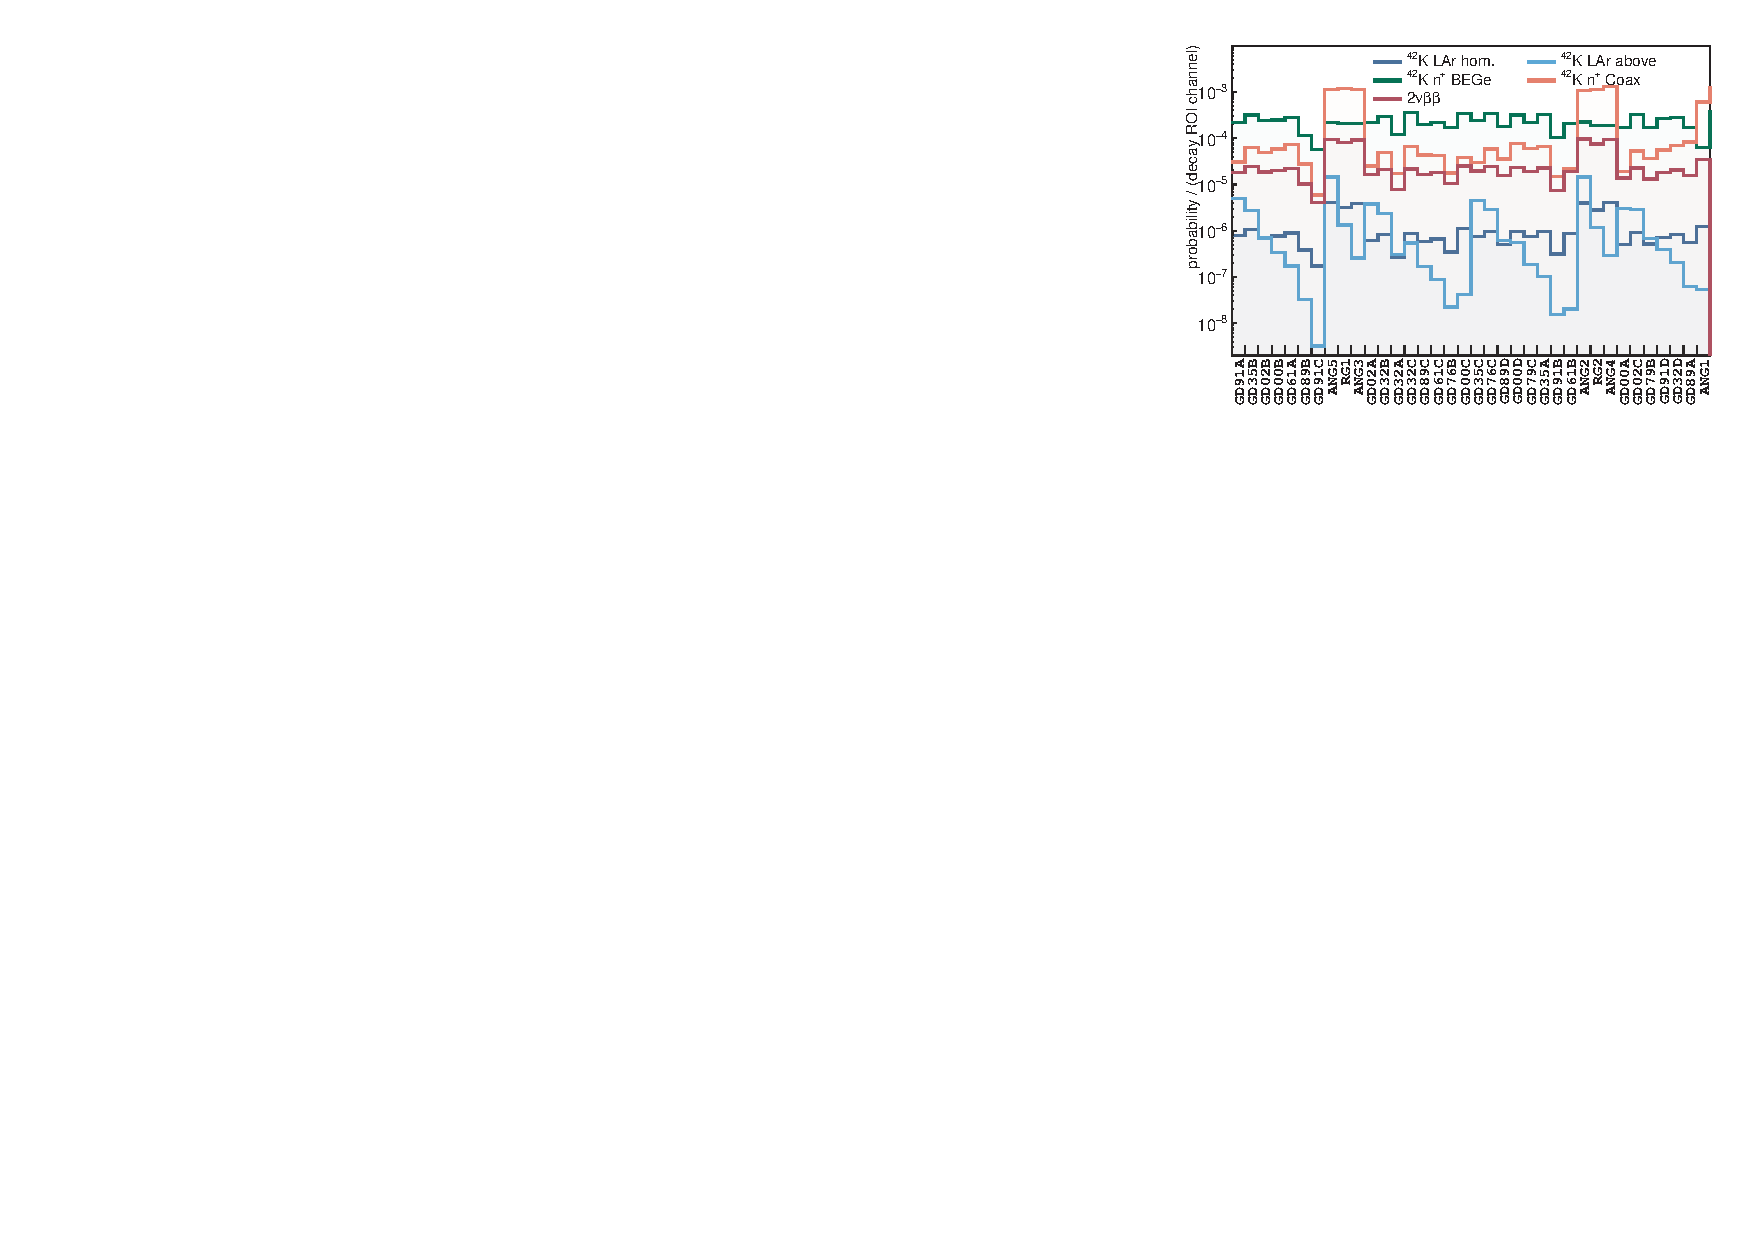
\includegraphics[width=0.45\textwidth]{plots/bkg/raw/ph2/pdfs/kmodel-pdfs-K42-long.pdf}}

  \caption{%
    From (a) to (e): pdfs in the full energy domain. The pdfs for the
    \enrGeII\ ($\enrBEGeII + \enrCoaxII$) (in fully opaque colors)
    and the \enrGeII\ (in shaded colors) data sets relative to different
    background sources. For visualization purposes a variable binning is
    adopted. (f) pdfs per detector channel for the \kvz\ \g\ line.
    All pdfs are normalized to the number of simulated primary decays.
  }\label{fig:bkg:raw:ph2:pdfs:gmodel}
\end{figure}

% vim: tw=90
